\section{背景}
\label{sec:background}

我们先介绍 GPU 的性能特征与执行模型。
随后描述标准注意力实现，以及 \sysnameone。

\subsection{硬件特征}
\label{subsec:hardware}

\textbf{GPU 性能特征。}
GPU 由计算单元（如浮点运算单元）和内存层次结构组成。
大多数现代 GPU 都包含用于加速低精度矩阵乘的专用单元（如 Nvidia GPU 上用于 FP16/BF16 矩阵乘的 Tensor Core）。
其内存层次主要包括高带宽内存（HBM）和片上 SRAM（即共享内存）。
以 A100 为例：其 HBM 容量为 40-80GB，带宽为 1.5-2.0TB/s；同时有 108 个流式多处理器（SM），每个 SM 配有 192KB 片上 SRAM，估计带宽约 19TB/s~\citep{jia2018dissecting,
  jia2021dissecting}。
由于程序员无法直接控制 L2 缓存，在本文讨论中我们重点关注 HBM 与 SRAM。
% 片上 SRAM 的速度比 HBM 快一个数量级，但容量小很多个数量级。
% 随着专用计算（矩阵乘）相对内存速度越来越快~\citep{nvidia2017nvidia,nvidia2020nvidia,nvidia2022nvidia}，
% 算子越来越受内存（HBM）访问瓶颈限制。
% 因此更应充分利用快速 SRAM。

\textbf{执行模型。}
GPU 使用大量线程来执行一个操作（称为 kernel）。
线程被组织为 thread block，并调度到流式多处理器（SM）上运行。
在每个 thread block 内，线程又分组为 warp（每组 32 个线程）。
同一 warp 内线程可通过快速 shuffle 指令通信，或协同完成矩阵乘。
同一 thread block 中不同 warp 可通过读写共享内存进行通信。
每个 kernel 从 HBM 将输入加载到寄存器和 SRAM，完成计算后再把输出写回 HBM。

\subsection{标准注意力实现}
\label{subsec:standard_attn}

给定输入序列 $\vQ, \vK, \vV \in \mathbb{R}^{N \times d}$，其中 $N$ 是序列长度、$d$ 是头维度，我们要计算注意力输出 $\vO \in \mathbb{R}^{N \times d}$：
\begin{equation*}
  \vS = \vQ \vK^\top \in \mathbb{R}^{N \times N}, \quad \vP = \softmax(\vS) \in \mathbb{R}^{N \times N}, \quad \vO = \vP\vV \in \mathbb{R}^{N \times d},
\end{equation*}
其中 $\softmax$ 按行应用。\footnote{为便于说明，我们省略了 $\vQ\vK^\top$ 的缩放（通常为 $1/\mathrm{d}$），以及可选地施加在 $\vS$ 上的逐元素掩码和/或施加在 $\vP$ 上的 dropout。}
对于多头注意力（MHA），同样的计算会在多个头上并行执行，并在 batch 维度（输入序列数）上并行。

注意力的反向传播如下。
设 $\vdO \in \mathbb{R}^{N \times d}$ 为某个损失函数对 $\vO$ 的梯度，则由链式法则（即反向传播）有：
\begin{align*}
  \vdV &= \vP^\top \vdO \in \mathbb{R}^{N \times d} \\
  \vdP &= \vdO \vV^\top \in \mathbb{R}^{N \times N} \\
  \vdS &= \dsoftmax (\vdP) \in \mathbb{R}^{N \times N} \\
  \vdQ &= \vdS \vK \in \mathbb{R}^{N \times d} \\
  \vdK &= \vQ \vdS^\top \in \mathbb{R}^{N \times d},
\end{align*}
其中 $\dsoftmax$ 是按行 softmax 的梯度（反向传播）。
可推得：若对某向量 $s$ 有 $p=\softmax(s)$，在输出梯度为 $dp$ 时，输入梯度为 $ds=(\diag(p)-pp^\top)dp$。

标准注意力实现会将矩阵 $\vS$ 与 $\vP$ 物化到 HBM，这需要 $O(N^2)$ 内存。
通常 $N \gg d$（典型地 $N$ 在 1k--8k 数量级，$d$ 在 64--128 左右）。
标准实现会先 (1) 调用矩阵乘（GEMM）子程序计算 $\vS=\vQ\vK^\top$ 并写入 HBM；再 (2) 从 HBM 读取 $\vS$ 计算 softmax 并将结果 $\vP$ 写回 HBM；最后 (3) 调用 GEMM 得到 $\vO=\vP\vV$。
由于多数操作受内存带宽限制，大量内存访问会直接导致较慢的实际运行时间。
此外，因为必须物化 $\vS$ 和 $\vP$，所需内存为 $O(N^2)$。
并且为了在反向传播中计算梯度，还必须保存 $\vP \in \mathbb{R}^{N\times N}$。

\subsection{\sysnameone}
\label{subsec:flashv1}

为了在 GPU 等硬件加速器上加速注意力，\citep{dao2022flashattention} 提出了在保持输出不变（无近似）的前提下减少内存读写的算法。

\subsubsection{前向传播}
\sysnameone 采用经典的分块（tiling）技术来减少内存 IO：
(1) 将输入块从 HBM 读入 SRAM；(2) 对该块计算注意力；(3) 更新输出且不把大型中间矩阵 $\vS$ 与 $\vP$ 写回 HBM。
由于 softmax 会耦合整行或行块，在线 softmax~\citep{milakov2018online, rabe2021self} 可将注意力计算拆成多个块，并在末端对各块输出重标定，从而得到正确结果（无近似）。
通过显著减少内存读写，\sysnameone 相对优化后的基线注意力实现可获得 2-4$\times$ 的端到端加速。

我们介绍在线 softmax 技术~\citep{milakov2018online} 及其在注意力中的用法~\citep{rabe2021self}。
为简化起见，仅考虑注意力矩阵 $\vS$ 的一个行块，形如
$\begin{bmatrix} \vS^{(1)} & \vS^{(2)} \end{bmatrix}$，其中
$\vS^{(1)},\vS^{(2)} \in \mathbb{R}^{B_r\times B_c}$，$B_r,B_c$ 分别为行块和列块大小。
我们希望计算这个行块的 softmax，并与 value 相乘，value 形如
$\begin{bmatrix} \vV^{(1)} \\ \vV^{(2)} \end{bmatrix}$，其中
$\vV^{(1)},\vV^{(2)} \in \mathbb{R}^{B_c\times d}$。
标准 softmax 计算如下：
\begin{align*}
  m &= \max(\mathrm{rowmax}(\vS^{(1)}), \mathrm{rowmax}(\vS^{(2)})) \in \mathbb{R}^{B_r}  \\
  \ell &= \mathrm{rowsum}(e^{\vS^{(1)} - m}) + \mathrm{rowsum}(e^{\vS^{(2)} - m}) \in \mathbb{R}^{B_r}  \\
  \vP &= \begin{bmatrix} \vP^{(1)} & \vP^{(2)} \end{bmatrix} = \diag(\ell)^{-1}\begin{bmatrix} e^{\vS^{(1)} - m} & e^{\vS^{(2)} - m} \end{bmatrix} \in \mathbb{R}^{B_r \times 2B_c} \\
  \vO &= \begin{bmatrix} \vP^{(1)} & \vP^{(2)} \end{bmatrix} \begin{bmatrix} \vV^{(1)} \\ \vV^{(2)} \end{bmatrix} = \diag(\ell)^{-1} e^{\vS^{(1)} - m} \vV^{(1)} + e^{\vS^{(2)} - m} \vV^{(2)} \in \mathbb{R}^{B_r \times d}.
\end{align*}
在线 softmax 则先按块计算“局部”softmax，再在末端重标定得到正确输出：
\begin{align*}
  m^{(1)} &= \mathrm{rowmax}(\vS^{(1)})  \in \mathbb{R}^{B_r}\\
  \ell^{(1)} &= \mathrm{rowsum}(e^{\vS^{(1)} - m^{(1)}}) \in \mathbb{R}^{B_r} \\
  \tilde{\vP}^{(1)} &= \diag(\ell^{(1)})^{-1} e^{\vS^{(1)} - m^{(1)}} \in \mathbb{R}^{B_r \times B_c}\\
  \vO^{(1)} &= \tilde{\vP}^{(1)} \vV^{(1)} = \diag(\ell^{(1)})^{-1} e^{\vS^{(1)} - m^{(1)}} \vV^{(1)} \in \mathbb{R}^{B_r \times d}\\
  m^{(2)} &= \max(m^{(1)}, \mathrm{rowmax}(\vS^{(2)})) = m \\
  \ell^{(2)} &= e^{m^{(1)} - m^{(2)}} \ell^{(1)} + \mathrm{rowsum}(e^{\vS^{(2)} - m^{(2)}}) = \mathrm{rowsum}(e^{\vS^{(1)} - m}) + \mathrm{rowsum}(e^{\vS^{(2)} - m}) = \ell \\
  \tilde{\vP}^{(2)} &= \diag(\ell^{(2)})^{-1} e^{\vS^{(2)} - m^{(2)}} \\
  \vO^{(2)} &= \diag(\ell^{(1)} / \ell^{(2)})^{-1} \vO^{(1)} + \tilde{\vP}^{(2)} \vV^{(2)} = \diag(\ell^{(2)})^{-1} e^{s^{(1)} - m} \vV^{(1)} + \diag(\ell^{(2)})^{-1} e^{s^{(2)} - m} \vV^{(2)} = \vO.
\end{align*}

我们展示 \sysnameone 如何使用在线 softmax 来实现分块（\cref{fig:flash_attention_diagram}），从而减少内存读写。
\begin{figure}[ht]
  \centering
  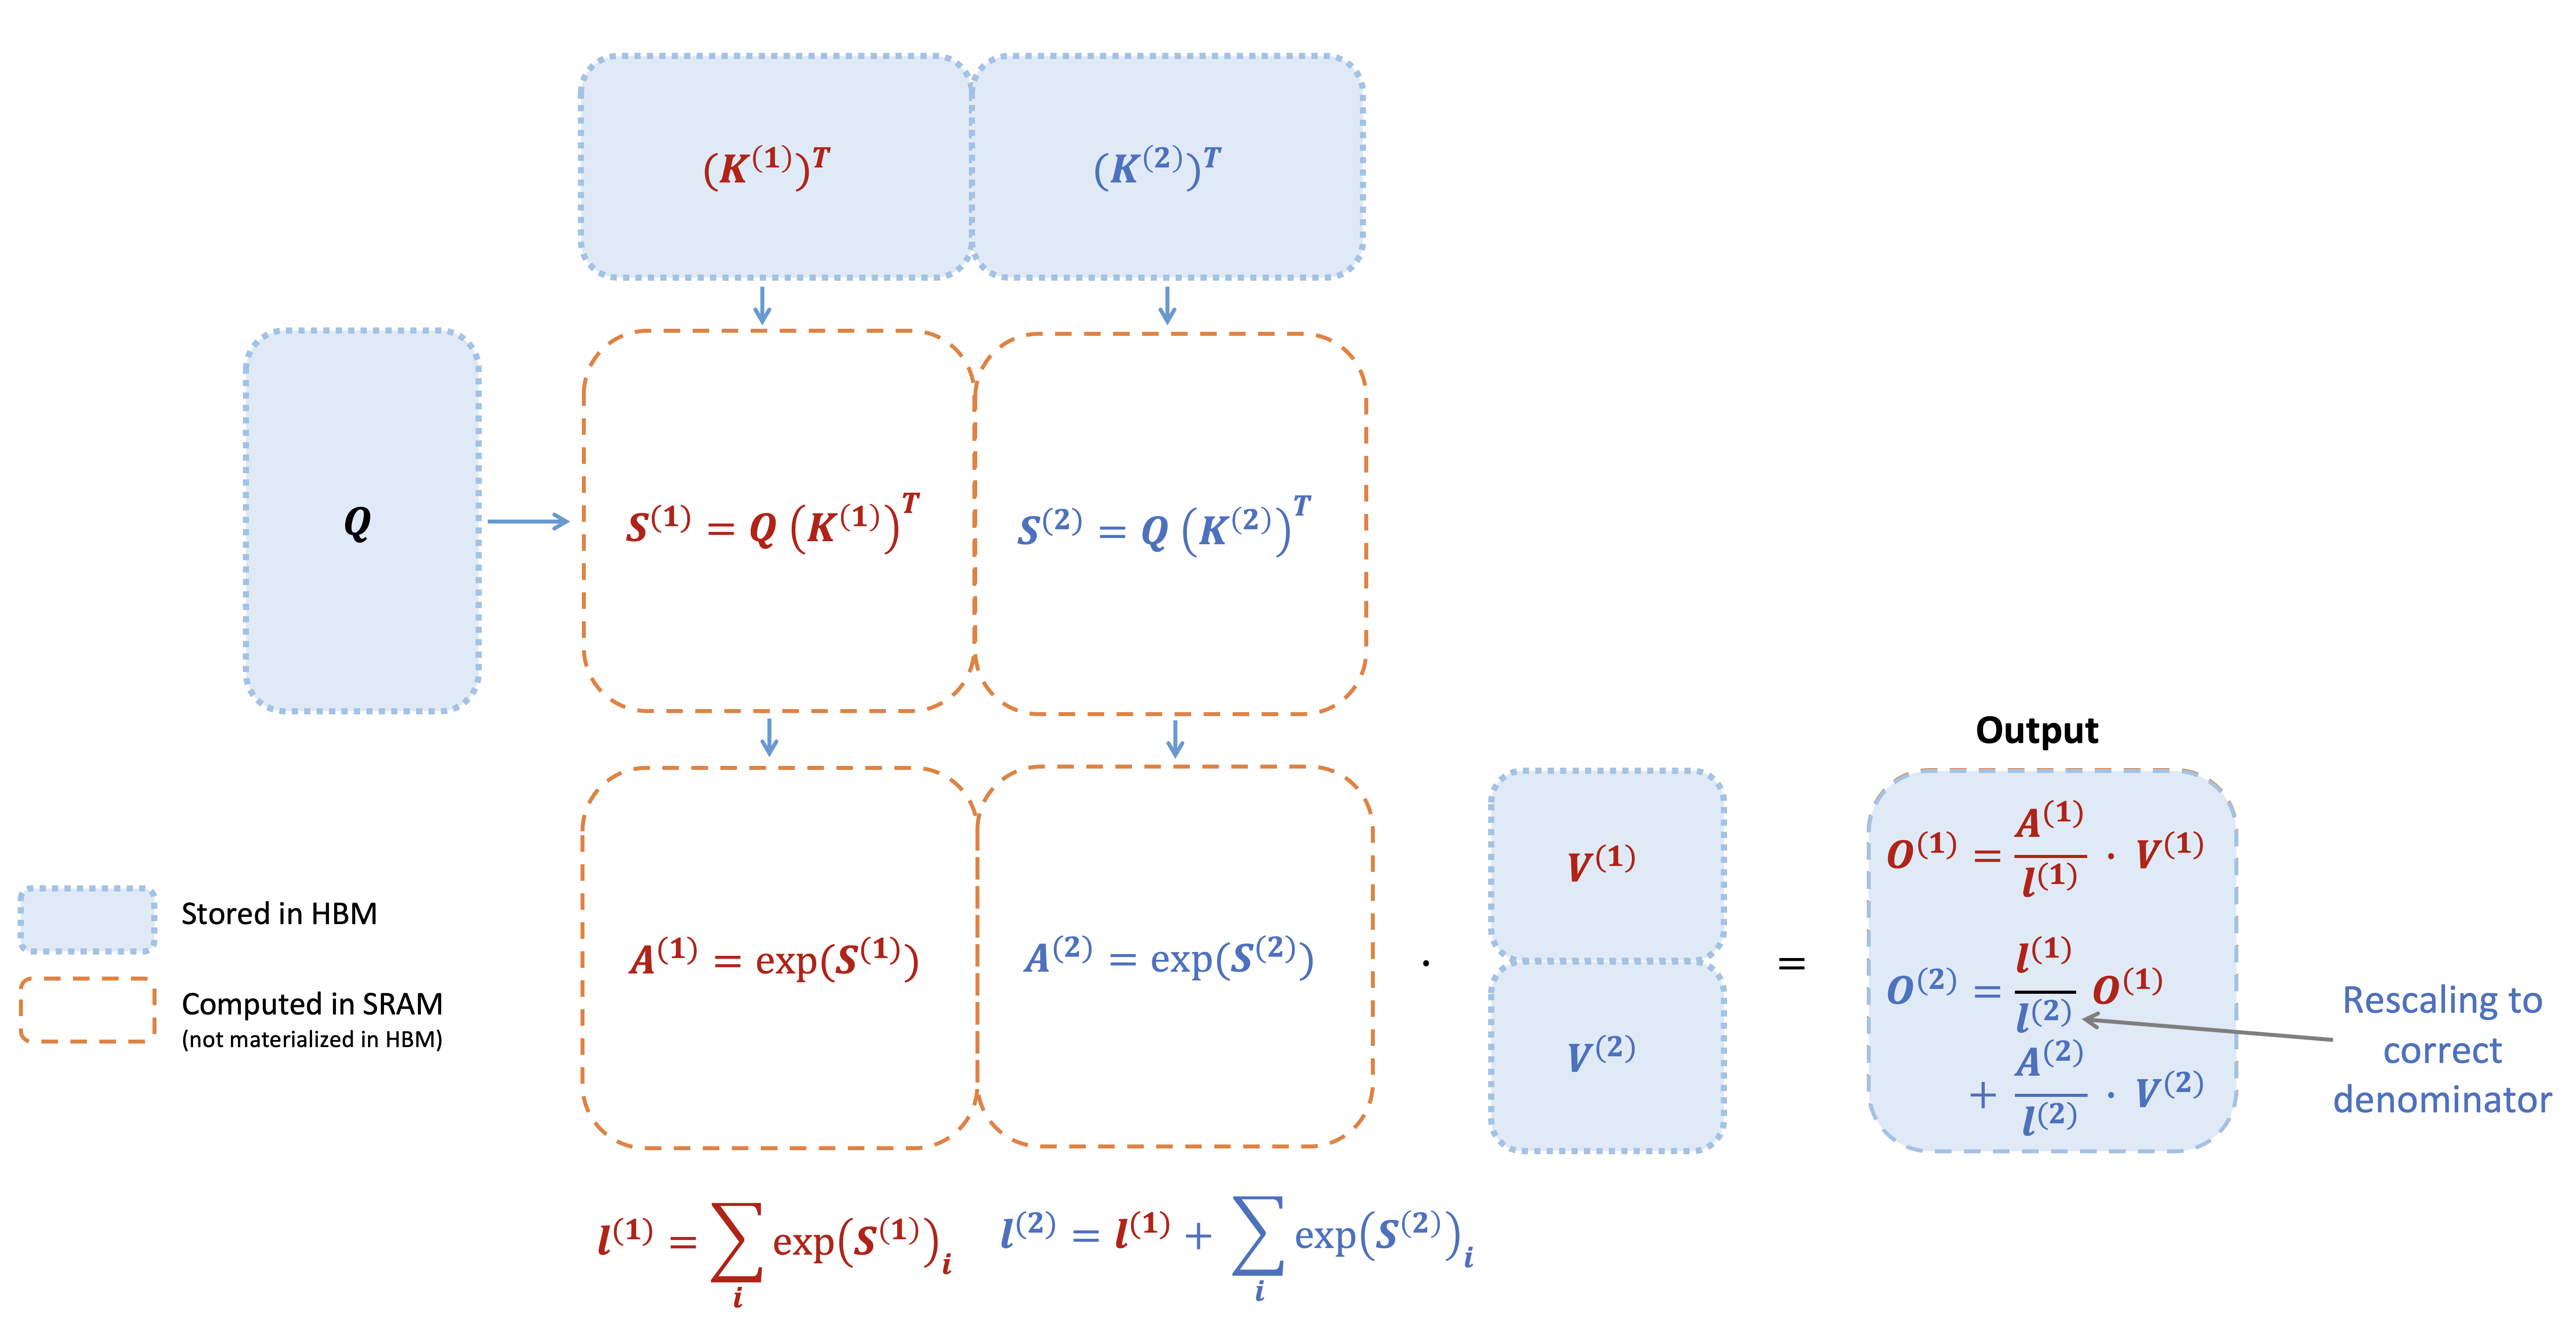
\includegraphics[width=0.9\textwidth]{figs/flash_attention_diagram.png}
  \caption{\label{fig:flash_attention_diagram}\sysnameone 前向传播示意图：当 key $\vK$ 被分成两个块、value $\vV$ 也被分成两个块时，
    通过分别对每个块计算注意力并对输出重标定，我们在末端得到正确结果，同时避免了中间矩阵 $\vS$ 与 $\vP$ 的高代价内存读写。
    图中为简化起见省略了 softmax 中“每个元素减去行最大值”的步骤。}
\end{figure}

\subsubsection{反向传播}
在反向传播中，一旦输入块 $\vQ,\vK,\vV$ 已加载到 SRAM，\sysnameone 会重计算注意力矩阵 $\vS$ 与 $\vP$，从而避免存储大型中间值。
由于不必保存大小为 $N\times N$ 的大矩阵 $\vS$ 和 $\vP$，\sysnameone 可根据序列长度获得 10-20$\times$ 的内存节省（所需内存随序列长度 $N$ 线性增长，而非二次增长）。
反向传播也因减少内存读写而获得 2-4$\times$ 的端到端加速。

反向传播将分块技术应用于 \cref{subsec:standard_attn} 的方程。
尽管从概念上看反向传播比前向更简单（没有 softmax 重标定），但实现上要复杂得多。
这是因为反向传播需要在 SRAM 中保留更多数值来执行 5 次矩阵乘，而前向仅需 2 次。

%%% Local Variables:
%%% mode: latex
%%% TeX-master: "../flash2"
%%% End:
